
\chapter{Related Work} \label{chap:related-work}
This chapter discusses several related research directions with similar motivations and objectives that we also aim to achieve, although with different approaches. Firstly, we describe similar works related specifically to HSMs, and lastly, we present cryptocurrency wallets, what they consist of, and how they relate to our work.

\section{Virtual HSMs} \label{sec:virtual-hsms}
Some attempts have been made to virtualize HSMs, intending to reduce the high costs of these infrastructures while maintaining acceptable performance and achieving security guarantees as close as those present in the physical HSM devices.

\subsection{SoftHSM} \label{subsec:softhsm}

\textit{SoftHSM} \cite{softhsmgithub} is part of the OpenDNSSEC project \cite{softhsm} and was one of the first successful attempts to virtualize an HSM. Currently in the second version, specifically in 2.1.13, it is an open-source project still used today in testing environments, emulating an HSM for clients incapable of buying an expensive physical HSM. The software was implemented in the C++ language, and its features are accessible through a PKCS\#11 interface \cite{pkcs11spec}, which, among other functionalities, allows generating keys, issuing signatures, and performing encryption/decryption. However, since this system runs only locally on a single machine, it offers no real security guarantees and should only be used for testing purposes.


\subsection{pmHSM} \label{subsec:pmhsm}

\textit{Poor Man's Hardware Security Module} or \textit{pmHSM} \cite{pmhsm}, was also developed by DNSSEC and provides the same functionalities as SoftHSM; however, it offers better security guarantees with a different approach. To improve security and availability while maintaining the idea of virtualizing an HSM, the system was implemented as a distributed solution using threshold cryptography.

\begin{figure}[h]
    \begin{center}
        \resizebox{60mm}{!}{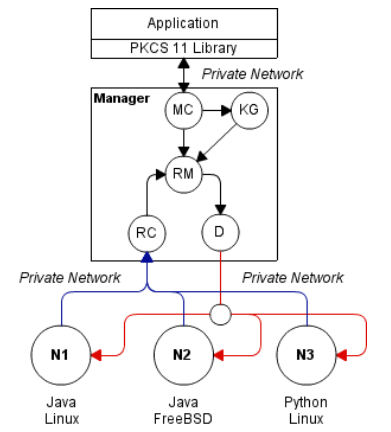
\includegraphics[]{3.pmhsm-arch}}
    \end{center}
    \caption{pmHSM architecture \cite{pmhsm}.}
    \label{fig:3.pmhsm-arch}
\end{figure}

The architecture of this virtual HSM is divided into three main layers, depicted in Figure \ref{fig:3.pmhsm-arch}: \textit{(i)} the \textit{application} that calls the functions of the PKCS\#11 API and translates them into messages to be sent to the next layer; (ii) the \textit{manager} that is responsible for receiving the requests from the application (e.g., signature, encryption, key generation), publishing them to the nodes and also waiting for their \textit{k} out-of \textit{n} responses, for instance, in case of a signing request, the nodes would send back to the manager a signature share; (iii) the \textit{shareholder} nodes correspond to the different replicas that communicate with the manager (in a \textit{publisher-subscribe} fashion), which receive the necessary information to complete the corresponding request (e.g., a document to sign in a signing request). 

In addition to the communications being transmitted synchronously between the servers, the main drawback of this work is that it is not a fully distributed solution. The manager acts as a trusted entity, sending and receiving sensitive cryptographic information, making it a single point of failure since the system depends on its honesty and availability. If an adversary manages to corrupt it, they can control everything and tamper with the messages as they see fit. Two protocols that would be directly affected by a Byzantine fault from the manager are: the key generation protocol, since the manager is responsible for generating the key and consequently possesses the full key and all its shares, given that it also has to create the corresponding shares using Shamir's secret sharing and also distribute them through the nodes; and the threshold signature scheme, considering that the private keys can be controlled by an adversary as well as all the signature shares that are received from the nodes.

Another weakness corresponds to the signature scheme employed, namely the threshold RSA signature scheme proposed by Victor Shoup \cite{practicalthresholdsignatures}, which is not as efficient as other recent protocols, not only due to the algorithm itself but also due to the need of bigger keys to achieve the same security level that other algorithms can achieve with smaller keys, as its the case of Schnorr and BLS, discussed in Section \ref{subsec:threshold-signatures}.

\subsection{Hardware-backed Virtual HSM} \label{subsec:rosahsm}

\textit{VirtualHSM} \cite{rosahsmthesis} corresponds to a project that developed a virtualized HSM supported by modern attestation-based trusted hardware in commodity CPUs to ensure privacy and reliability. The primary focus of this work was to develop a virtual HSM that could offer security guarantees similar to physical HSMs and achieve high availability through techniques like cloud-of-clouds replication on nodes equipped with trusted hardware. The proposed solution involves creating a virtualized and distributed HSM on the cloud, specifically utilizing Intel Software Guard Extension (SGX) \cite{intelsgx} enabled nodes for private key management, preserving the virtual HSM state, even if the node shuts down, by using an encrypted persistent data storage outside of the enclave, i.e., physical memory regions isolated from the rest of the system, including the operating system and hypervisor, where code can run with confidentiality and integrity guarantees provided by the hardware, in this case, Intel SGX. 

The downsides of this project are that it still requires the usage of trusted hardware and, although the authors claim it to be a distributed solution, it is more of a replicated centralized solution. This is because the HSM operations are performed on a single machine and, consequently, the security of the system is dependent exclusively on that machine's safety, specifically, the secure channels and the Intel SGX, as illustrated in Figure \ref{fig:3.rosahsm}. After a pre-defined number of executions resulting in state changes on a specific HSM machine, a batch with these changes is submitted to the other replicas.

\begin{figure}[h]
    \begin{center}
        \resizebox{130mm}{!}{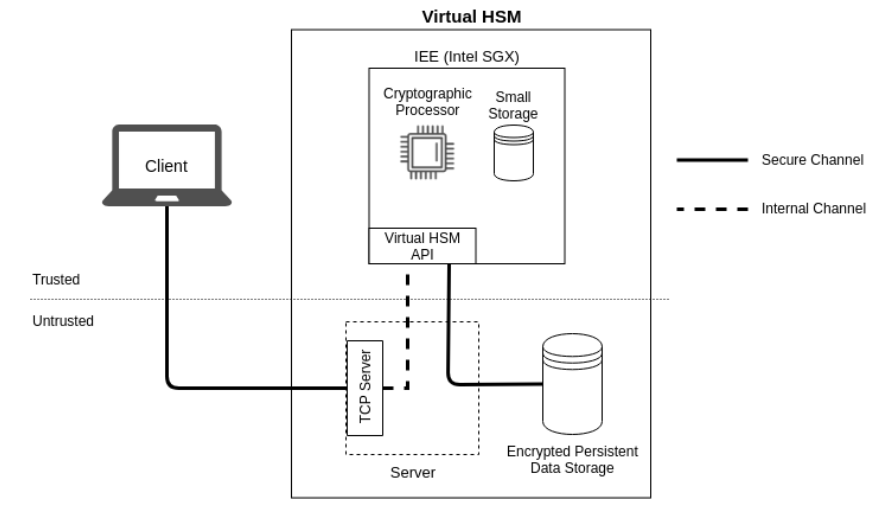
\includegraphics[]{3.rosahsm}}
    \end{center}
    \caption{VirtualHSM system architecture. The server acts as a proxy to securely connect the client with the Intel SGX, and this with the persistent storage \cite{rosahsmthesis}.}
    \label{fig:3.rosahsm}
\end{figure}


\subsection{Cloud HSMs} \label{subsec:cloudhsms}

\textit{Cloud HSM solutions} \cite{physicalvscloudhsm} enable users to quickly integrate high-performance cryptographic operations and secure key storage into their applications without the need to maintain on-premises appliances. Leading cloud providers offer fully managed HSM solutions that customers access via APIs and management platforms, the most popular of which are AWS CloudHSM, Azure Dedicated HSM, and Google Cloud HSM. These types of solutions offer no upfront hardware costs as the provider manages and operates the physical HSM infrastructure, provides a usage-based billing model where customers pay only for the time they use the HSM services, and delivers a seamless scaling through the provider as well as built-in high availability and redundancy. However, typically, these solutions work with physical devices and lead to customers having less visibility and control over the physical HSM devices owned by the provider. This can be a critical decision factor since the processed data is sensitive, and trusting a third party to store this type of information is always difficult. Moreover, even if there are no upfront costs to use this type of solution, but only an hourly fee for each HSM that is launched until it is terminated, the costs can also scale quickly. Using the AWS CloudHSM as an example, an HSM in Paris has an hourly price of \$2.18 per HSM, resulting, for a single HSM, in a monthly bill of \$1,591.40 \cite{awscloudhsmpricing}.


\section{Cryptocurrency Wallets} \label{sec:crypto-wallets}

Cryptocurrency wallets \cite{cryptowalletreview} provide customers the ability to send and receive digital currency through interaction with blockchains and can be referred to as software or hardware wallets:
\begin{itemize}
    \item \textbf{Software wallets:} Downloadable software programs that can be hot or cold, depending on whether it is connected to the Internet. Since nothing on the Internet is 100\% safe and money stored in a hot wallet is always vulnerable to theft, viruses, or loss due to software faults, these wallets are also more likely to be hacked. Moreover, these wallets can also operate in the cloud, and although convenient to access, it means that a third party controls the private and public keys stored in these wallets.
    \item \textbf{Hardware wallets:} Physical vaults that hold private keys on a hard drive specifically designed for that purpose. Although hardware wallets make transactions online, public and private keys are saved offline. 
\end{itemize}

These wallets, regardless of their type, should always provide a set of important features that complement their basic functionality of storing private keys and signing transactions, which include:
\begin{itemize}
    \item \textbf{Account creation:} Generate a pair of keys, a private key used to sign transactions, and a public key that acts as a public address, like an account number, used to interact with a blockchain, such as for accessing transactions associated with that address;
    \item \textbf{Key management:} Store and protect private keys. In a non-hosted wallet, the private keys are in the account owner's possession, while in a hosted wallet, a third party handles this task, and the account owner is unaware of the private keys. The organization handles the sending, receiving, and cryptocurrency storage on his behalf. Nonetheless, certain establishments do not keep personal keys; instead, they request them when needed;
    \item \textbf{View cryptocurrency balance and transactions:} This information is obtained from the blockchain using the user's public key;
    \item \textbf{User authorization:} Allow the user to access the wallet, which can be simply a PIN (Personal Identification Number) associated with the private key of the respective account;
    \item \textbf{User anonymity:} Send and receive funds anonymously by blockchain users. Anonymity is available on three levels: full, half, or less than half. A completely anonymous wallet does not request user information, unlike financial institutions that require users to register with all their personal information. If the mail ID is the only data needed to create or recover a password from a wallet, then the wallet is said to be half anonymous. Significantly less anonymous wallets collect a significant amount of data about their users;
    \item \textbf{Multicurrency support:} Enables users to use multiple cryptocurrencies inside of a single wallet concurrently;
    \item \textbf{Submit transactions:} Allows customers to move funds. The wallet signs the transaction with the private key, while the public key corresponds to the account of the receiver;
    \item \textbf{Wallet recovery:} If users forget their password or PIN, to prevent the coins from being lost forever, a widely used method is the seed phrase, a set of 12-24 random words used to recover access to the wallet.
\end{itemize}

Blockchains depend on cryptographic operations, and safeguarding private keys is imperative to protect the security of blockchain processes. Cryptocurrency wallets, as previously mentioned, are the connection to blockchains, and their main responsibilities are performing cryptographic operations and storing and protecting private keys, just like HSMs. The synergy between these technologies can contribute to improving the security of these systems; however, as stated before, physical HSMs are expensive devices, and since there are many cheaper centralized alternatives dedicated to cryptocurrency wallets, the investment might not compensate. This union is mentioned in some papers \cite{velinkhsmwallet,hsmbasedewalleteth}, where they use physical HSMs to secure private keys and to verify the user's identity through a PIN.

The theft of blockchain-based digital assets is a frequent reality \cite{cryptothefts2024}, and honest users should be protected from these events using different strategies. A secure cryptocurrency wallet should allow its user to divide their signing key among several devices and need all of them, or just a subset to complete a transaction, not enabling any single party to possess the signing key. Beyond splitting the key into multiple parts, the signature protocol being distributed will also allow each party to sign independently, using their portion of the key, where the final signature will be the combination of all the individual signatures. These types of systems can be achieved through threshold cryptography. 

Although there are publications regarding threshold wallets~\cite{goldfederwallets,bip32wallet,unstoppablewallet,proactivewallet}, their focus is primarily on threshold ECDSA signatures~\cite{gennaro18,damgard20}, which tend to have lower performance compared to non-interactive protocols due to the need for multiple communication rounds. Non-interactive signature schemes recently supported by blockchains, such as Schnorr and BLS, along with underlying wallet implementation features, such as, server recovery, server replacement, and secret resharing, are important characteristics of such distributed systems not addressed in these proposals. There are also proprietary solutions that implement threshold wallets; however, they do not disclose much information about the technologies and protocols used to achieve their results. Zengo \cite{zengowallet} and Blockdaemon Wallet \cite{blockdaemonwallet} are examples of organizations that developed solutions to protect digital assets by distributing operations using threshold cryptography, where both use Multi-Party Computation (MPC) to provide the security foundation for the corresponding services. The former uses an open-sourced MPC library maintained by the same company, while the latter uses a patented ``Advanced MPC protocol."



\section{Discussion} \label{sec:relatedwork-discussion}

In this chapter, we introduced the most recognized attempts to virtualize an HSM. SoftHSM implements a local solution for a virtual HSM, achieving a performance 15 to 20 times faster than the pmHSM, according to a comparison made by the authors. However, the first solution did not provide security guarantees, which was improved by the second version of the system by making it distributed, contributing to this difference in the obtained results. Additionally, the project developed by Miguel Rosa (VirtualHSM) achieved even better results mainly due to the fact that he uses dedicated hardware to perform cryptographic operations on a single machine, as in SoftHSM. The difference is that this work achieves necessary security guarantees, such as privacy, by using a trusted execution environment and availability by replicating the data among the servers.

Nevertheless, all the proposals present centralized or semi-distributed solutions, where some security properties are missing or are implemented differently than we intend to implement in our solution. As attempted by DNSSEC, the key to substantially lowering the costs of HSM infrastructures is not to try to beat the performance of the physical devices but to achieve the same security guarantees using other strategies. Therefore, we intend to implement a fully distributed solution, without any dependency on dedicated cryptographic hardware, that addresses the limitations of previous solutions, achieving the required security properties, including confidentiality, availability, and integrity, all in one system using threshold cryptography as well as a BFT SMR system, providing fault-tolerant features in the presence of Byzantine faults, which neither of the related works also offered. All these characteristics contribute to making a practical and realistic system in the real world.

Regarding cryptocurrency wallets, the objective is to develop secure implementations that can efficiently protect the digital assets of its users. The threshold versions of these wallets, although they can still be vulnerable to several attacks \cite{attackingthresholdwallets} if not correctly implemented, by using threshold cryptography to protect the keys, such as using secret sharing and also threshold signature schemes, the key is distributed in shares among different servers, requiring that an adversary compromises several of them to recover the private key.

\begin{figure}[h]
    \begin{center}
        \resizebox{120mm}{!}{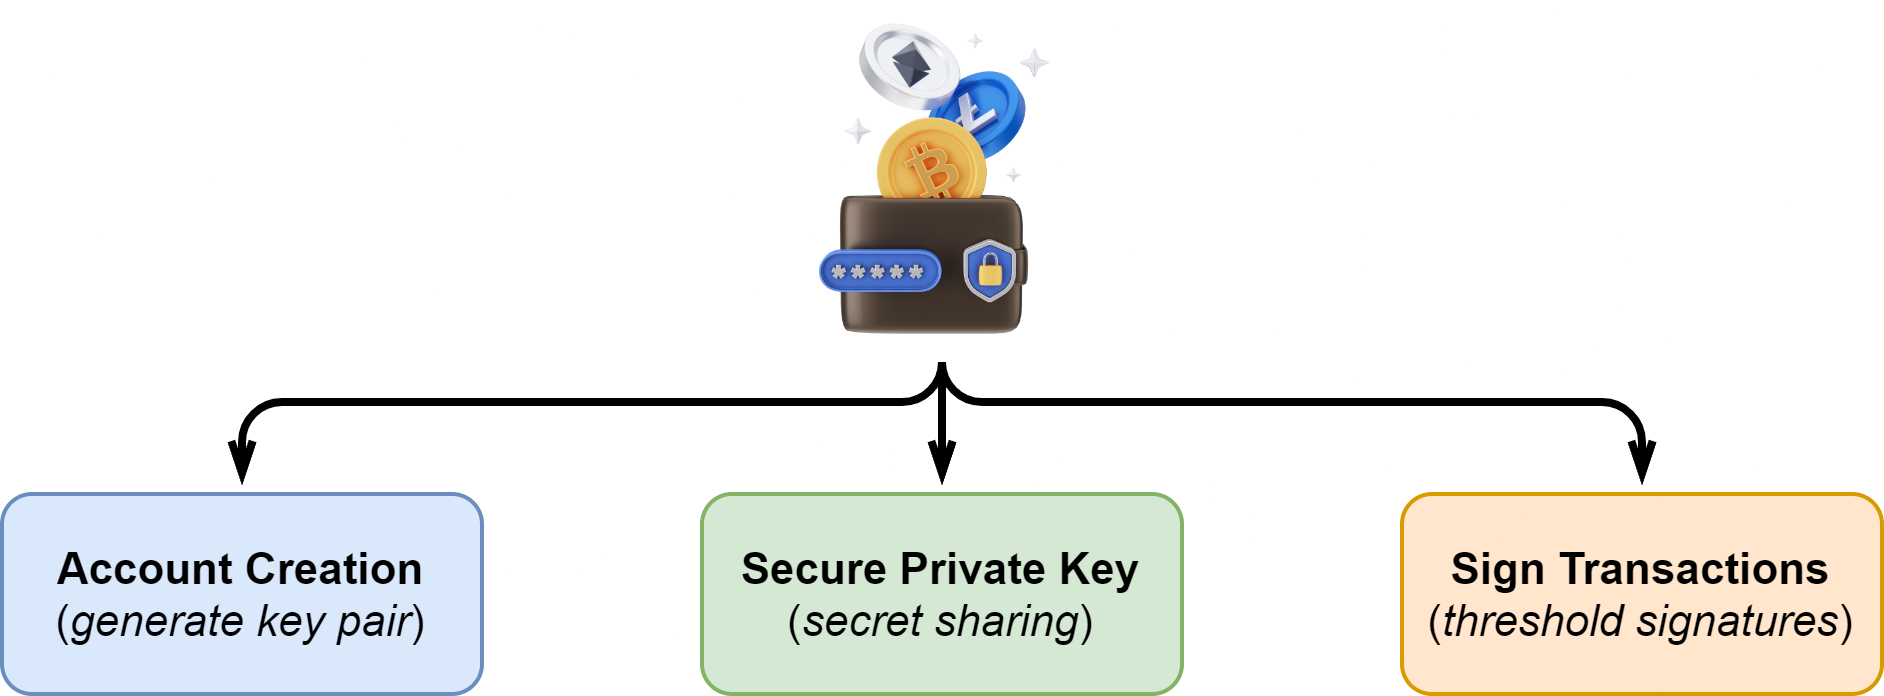
\includegraphics[]{3.cryptowalletfeatures}}
    \end{center}
    \caption{Cryptocurrency wallets main features supported by our system.}
    \label{fig:3.cryptowalletfeatures}
\end{figure}

Our open-sourced implementation, unlike proprietary solutions that require MPC protocols and public proposals that focus mostly on a single interactive signature scheme while neglecting important BFT SMR features for this type of system, represents a perfect use case for these wallets since it provides all the necessary threshold protocols to develop the most important functionalities, namely, account creation through generating keys in a fully distributed manner, safe storage of the private keys using secret sharing techniques, and transaction signing using only the shares of the key.

%\LIMPA